\label{sec:design}
The Liaison System is created to assure that the correct data collected from a microcontrollers is received correctly by the end user.
To achieve this, the system uses four equal but distinct microcontrollers, an internal voting system to assure that if any of the microcontrollers
disagree, it is marked as malfunctioning and is no longer allowed to send output. The output from the Liaison is extended with a system status
code that tells the end user if any of the microcontrollers are damaged, and the signal is then enhanced with an error correcting code such that
we can be more certain that the signal is not distorted on its way to the reciever.

\begin{figure}[h]
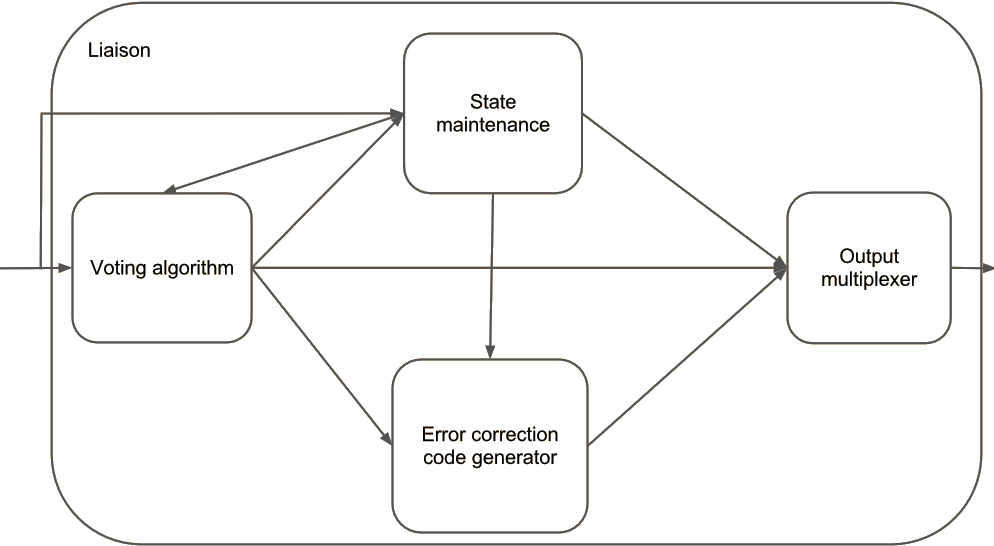
\includegraphics[width=15cm]{design/fig_overview}
\caption{Modules overview}
\label{fig:overview}
\end{figure}

As we can see from \autoref{fig:overview}, the internals of the Liaison can be modeled as four different pieces of hardware, each providing a
nessesary service to the system.

\subsection{System Assumptions}
\todo[inline]{Write about the assumptions (maybe not here, but somewhere)}


\subsection{Voting algorithm}
The system needs to distinguish between the working and the
malfunctioning microcontrollers. To do this, the voting module knows
what microcontrollers that has shown sign of failure from earlier
voting, and it needs to vote for the majority result of working
microcontrollers. This modules receives input directly from the
microcontrollers, and it gets the current system state from the State
Maintainance module.

The algorithm in our design works by partitioning the microcontrollers
into two pairs. For the following explanation, the microcontrollers
will be labeled A, B, C and D, and the groups in the partition will be
labeled (A, B) and (C, D).

First, each group performs what will be referred to as a local
vote. The result from this local vote is tabulated in
\autoref{tab:localvote}.

\begin{table}[htbp]
  \centering
  \caption{Local vote between microcontroller pairs}
  \begin{tabular}{|c|c|}
    \hline
    \textbf{Condition} & \textbf{Result} \\ \hline
    MCU1 and MCU2 both untagged & MCU1 data $\wedge$ MCU2-data \\ \hline
    Only MCU1 untagged & MCU1 data \\ \hline
    Only MCU2 untagged & MCU2 data \\ \hline
    Both tagged   & 0 \\ \hline
  \end{tabular}
  \label{tab:localvote}
\end{table}

The local vote gives the majority vote between the two
microcontrollers. In the case of a tie, or both microcontrollers being
tagged as erroneous, the output from the vote is 0. 

The algorithm then proceeds by distinguishing between three different
scenarios. These scenarios are tabulated in
\autoref{tab:globalvote}. The condition in each row also implies that
none of the conditions in rows above it hold.

\begin{table}[htbp]
  \centering
  \caption{Final vote result}
  \begin{tabular}{|p{7cm}|c|}
    \hline
    \textbf{Condition} & \textbf{Result} \\ \hline
    A, B untagged and (A,B)-result is not a tie & (A, B)-result \\ \hline
    (C, D)-result is not a tie & (C, D)-result \\ \hline
    Neither pair is safe  & (A, B)-result $\vee$ (C, D)-result \\ \hline
  \end{tabular}
  \label{tab:globalvote}
\end{table}

First, it checks whether both A and B are untagged and have the same
data value. If this is the case, then the output from the local vote
of (A, B) will have two votes, which is enough to ensure either
majority or a tie no matter what the result from (C, D) is.

If this is not the case, then either A or B is faulty, and the (A,
B)-result represents at most one vote. If the (C, D)-result is not a
tie, then it represents two, one or zero votes to the (C, D)-result
without providing any votes which could strengthen the (A, B)-result.

\begin{itemize}
\item If the (C, D)-result represents two votes, it will 
\end{itemize}


If the (C, D)-result represents two votes, it is the majority result,
and if it represents zero votes the system is broken so it does not
matter what is voted. If the (C, D)-result represents only one vote,





To perform this voting, the voter arranges the input data from the microcontroller 


\subsection{State maintainance}
The State Maintainance module is responsible for all internal states
of the system. The system keeps track of what microcontrollers that
can no longer be trusted. This works by tagging those microcontrollers
were the signal differs from the voted signal from the Voter
module. When a microcontroller has been tagged, the tag is not cleared
until the entire system is reset.

This module also outputs a system status vector as part of the Liaison
output. This vector has one of four states as shown in
\autoref{tab:systemstatus}.  The output status is a direct mapping
from the internal tag-vector, and works simply as a lookup table.

At last, the State Maintainance module is also responsible for
counting what output is sent at each clock tick. Since we are
outputing a serial data stream where different sections of the stream
have different sources (data, status, ECC), we need to keep track of
the position of the current data bit.



\subsection{Error Correcting Code Generator}
To provide reliable output for long distance transmission of data, the
Liaison System was required to add an error correcting code (ECC) to
its data packets. As stated in \autoref{sec:problem}, the ECC should
be able to correct one bit errors and detect two bit errors. To
fulfill the first criteria, we use a (15, 11)
Hamming-code\cite{ecc}. Since the Liaison sends eleven data bits ---
eight for the voted data and three for the status --- using four
parity bits is sufficient to provide detection and correction for one
bit errors. To be able to detect two bit errors, one can use an extra
parity bit covering all the transmitted bits, including data, status
and the four other ECC bits. This final parity bit is called
SECDED-bit, since it makes the Hamming code a Single Error Correction
Double Error Detection code\cite{ecc}. For simlicity, we will refer to
this error correction code scheme as a (16, 11) Hamming code.

The Error Correcting Code Generator generates (16,11) Hamming code on
the fly and attaches the code at the end of the output stream. This
module uses information from the Voter to get the first w8 data bits
and information from the State Maintainance to get the status word. It
also uses information on current data bit position from the State
Maintainance module, since Hamming Code is generated using parity of
bits at specific positions\cite{ecc}.

When (16,11)-Hamming code is used, we are able to correct a single
error in the packet, but we are also able to detect up to two errors
in the same packet.  The first 4 bits in the Hamming code is used for
error correction of a single bit, and the additional bit adds the
ability to detect another error.

\subsection{Output Multiplexer}
Since the Liaison System needs to send output from each of the three other modules at specific clock cycles when specific events has occured, we need
a logic piece of hardware that can multiplex all modules and allways output the correct signal. The Output Multiplexer uses the position of current data bit
from the State Maintainance module to select what module to send data from.
